\begin{figure}[]
	\begin{subfigure}{\linewidth}
		\caption{}
		\centering
		% include first image
		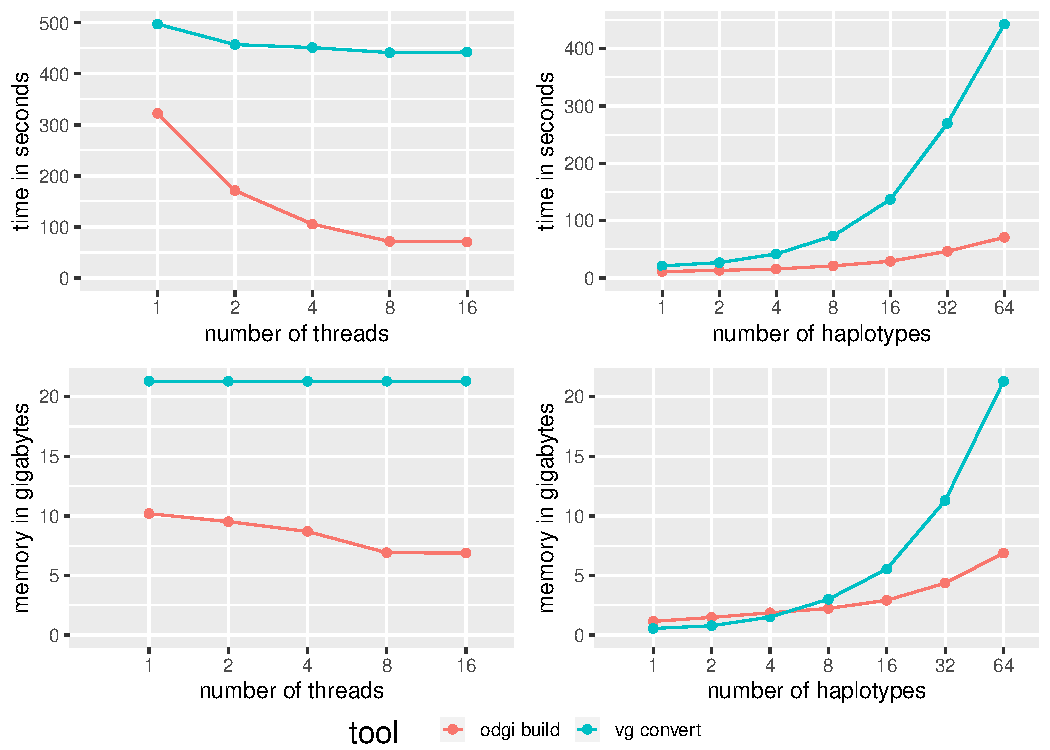
\includegraphics[width=1.0\linewidth, trim=0cm 1.25cm 0cm 0cm]{fig/performance/build_eval.pdf}
		\label{fig:eval-build}
	\end{subfigure}
	\begin{subfigure}{1\linewidth}
		\caption{}
		\centering
		% include fourth image
		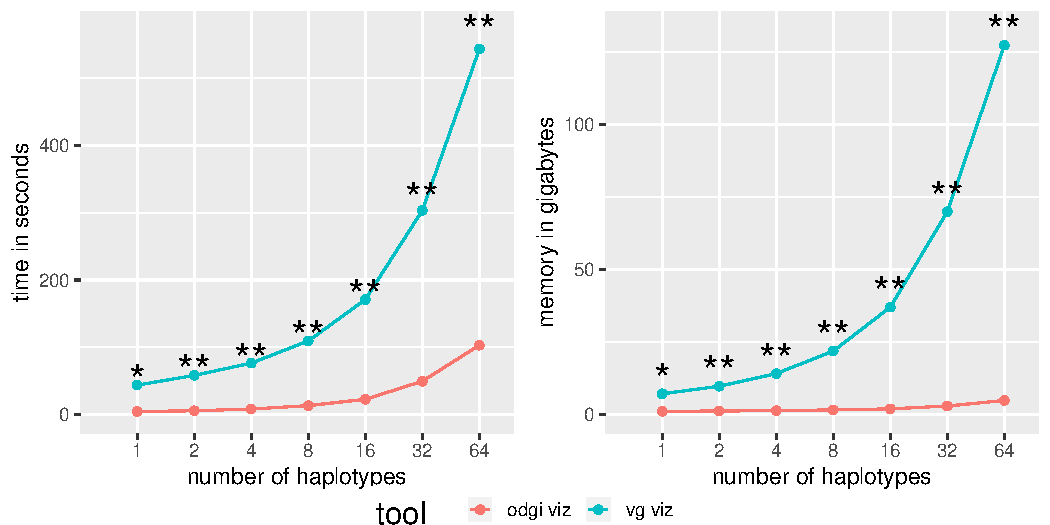
\includegraphics[width=\linewidth, trim=0cm 1.25cm 0cm 0cm]{fig/performance/viz_eval.pdf}
		\label{fig:eval-viz}
	\end{subfigure}
	\begin{subfigure}{\linewidth}
		\caption{}
		\centering
		% include second image
		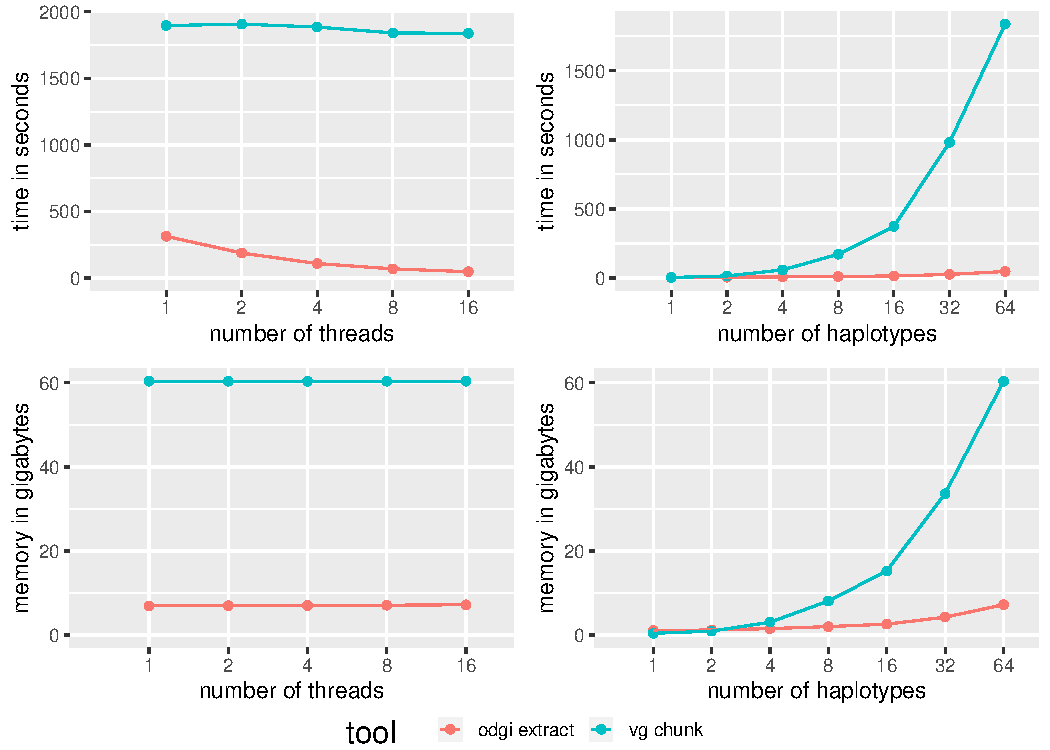
\includegraphics[width=\linewidth, trim=0cm 1.25cm 0cm 0cm]{fig/performance/extract_eval.pdf}
		\label{fig:eval-extract}
	\end{subfigure}
	\caption{TODO}
	\label{fig:evaluation}
\end{figure}
